\documentclass{ubicomp2011}
\usepackage{times}
\usepackage{url}
\usepackage{graphics}
\usepackage{color}
\usepackage[pdftex]{hyperref}
\hypersetup{%
pdftitle={Info@ITU}, pdfauthor={Egil Hansen, Jonas Rune Jensen}, pdfkeywords={ITU, BLIP, Android, Mandatory Assignment}, bookmarksnumbered, pdfstartview={FitH}, colorlinks,
citecolor=black, filecolor=black, linkcolor=black, urlcolor=black,
breaklinks=true, }
\newcommand{\comment}[1]{}
\definecolor{Orange}{rgb}{1,0.5,0}
\newcommand{\todo}[1]{\textsf{\textbf{\textcolor{Orange}{[[#1]]}}}}

%\pagenumbering{arabic}  % Arabic page numbers for submission.  Remove this line to eliminate page numbers for the camera ready copy

\begin{document}
% to make various LaTeX processors do the right thing with page size
\special{papersize=8.5in,11in}
\setlength{\paperheight}{11in}
\setlength{\paperwidth}{8.5in}
\setlength{\pdfpageheight}{\paperheight}
\setlength{\pdfpagewidth}{\paperwidth}

% use this command to override the default ACM copyright statement
% (e.g. for preprints). Remove for camera ready copy.
\toappear{}



\title{Info@ITU}
\numberofauthors{2}
\author{
  \alignauthor Egil Hansen\\
    \affaddr{IT University of Copenhagen}\\
    \email{ekri@itu.dk}
 \alignauthor Jonas Rune Jensen\\
    \affaddr{IT University of Copenhagen}\\
    \email{jrur@itu.dk}}

\maketitle

% \begin{abstract}
% \end{abstract}
\section{Introduction}

We decided to base our Info@ITU system on three main components, a Info@ITU Monitor (monitor), which tracks the user while inside ITU and displays information to the user when the user is close to a display, a Info@ITU Proxy (proxy) which sits between the monitor and the Android devices and keeps track of the devices that are entering and leaving ITU, and an Info@ITU App for tracking outside of ITU. This provides loose coupling between the components and in theory will allow us to scale up more easily.

\section{Info@ITU Monitor}

-areas:
Gapps
Blipmonitor
JCAFinfo
\section{Info@ITU Proxy}

The proxy is available at http://info-at-itu-proxy.appspot.com and provides the following service methods for the monitor and mobile devices:

\begin{itemize}
\item \texttt{entering?<BT MAC address>\&<Username>}\\
This method is used by the phone to tell the system that the phone is moving into ITU and to start tracking the it.
\item \texttt{leaving?<BT MAC address>}\\
This method is used by the phone to tell the system that the phone has left ITU and to stop tracking it.
\item \texttt{ping?<BT MAC address>}\\
This method should be used every XX minutes, after the phone has entered into ITU, to indicate to the system that the phone is still turned on and inside ITU.
\item \texttt{getallclients}\\
This method returns a JSON formatted aray of all clients that have been `checked in’ with the proxy.
\end{itemize}

The reason why we added the \texttt{ping} method is to handle the common scenario where the phone is out of range of ITU's BLIP sensors for a longe time, i.e. when the owner is in a meeting room or lecture hall, or if the owner has turned of his phone or the phone has simply run out of power. If the proxy stops receiving pings from the phone, we assume that the phone should no longer be tracked and can save resources on the monitor.

\subsection{Future Work}

A related feature to the \texttt{ping} method, which is not yet implemented, is a scheduled clean-up job, that searches through the list of `checked in' phones on the proxy and removes those who have not `pinged in' for 20 minutes.

Push notificaitons from the proxy to the monitor would also be natural extension, since it would lower the resources required and allow the monitor to be notified almost instantly when a new phone `checks in'. In the current solution, the monitor pulls from the server every 15 seconds to see if there are any new phones or phones that have left.

\section{Info@ITU App}

For our Info@ITU App we considered the problems with identification (who is actually using the Android device), battery life, and volatile state.

\paragraph{Identification}
This is an issue even if mobile phones are often very personal, since they could be shared between people, or more likely, a person could have a private profile and a public profile. So to identify the user of the phone, we ask the user to select one of his Google accounts when signing in to Info@ITU from his device. This also enable the scenario where a user switches between devices or is signed in with multiple devices, since we identify him and his devices by his Google ID, not by an MAC address.

\paragraph{Battery life}
This can quickly become an issue when both WiFi, GPS and Bluetooth radios are turned on. So we try to be as effective as possible, only turning on Bluetooth when the device is actually inside ITU.

\paragraph{Volatile state}
The volatile state of mobile devices must also be considered -- the user can choose to turn it of, the device can run out of battery, the user can turn of Bluetooth or GPS, other applications can turn of Bluetooth or GPS, all things we need to consider when building an app like this that relies on these.

The workflow of our App is illustrated in figure \ref{fig:android-app-activity-diagram}. Before we enter into the initial waiting state in the figure, the user is asked  to sign in to our application with a Google ID of his choice.

\begin{figure}[t]
\begin{center}
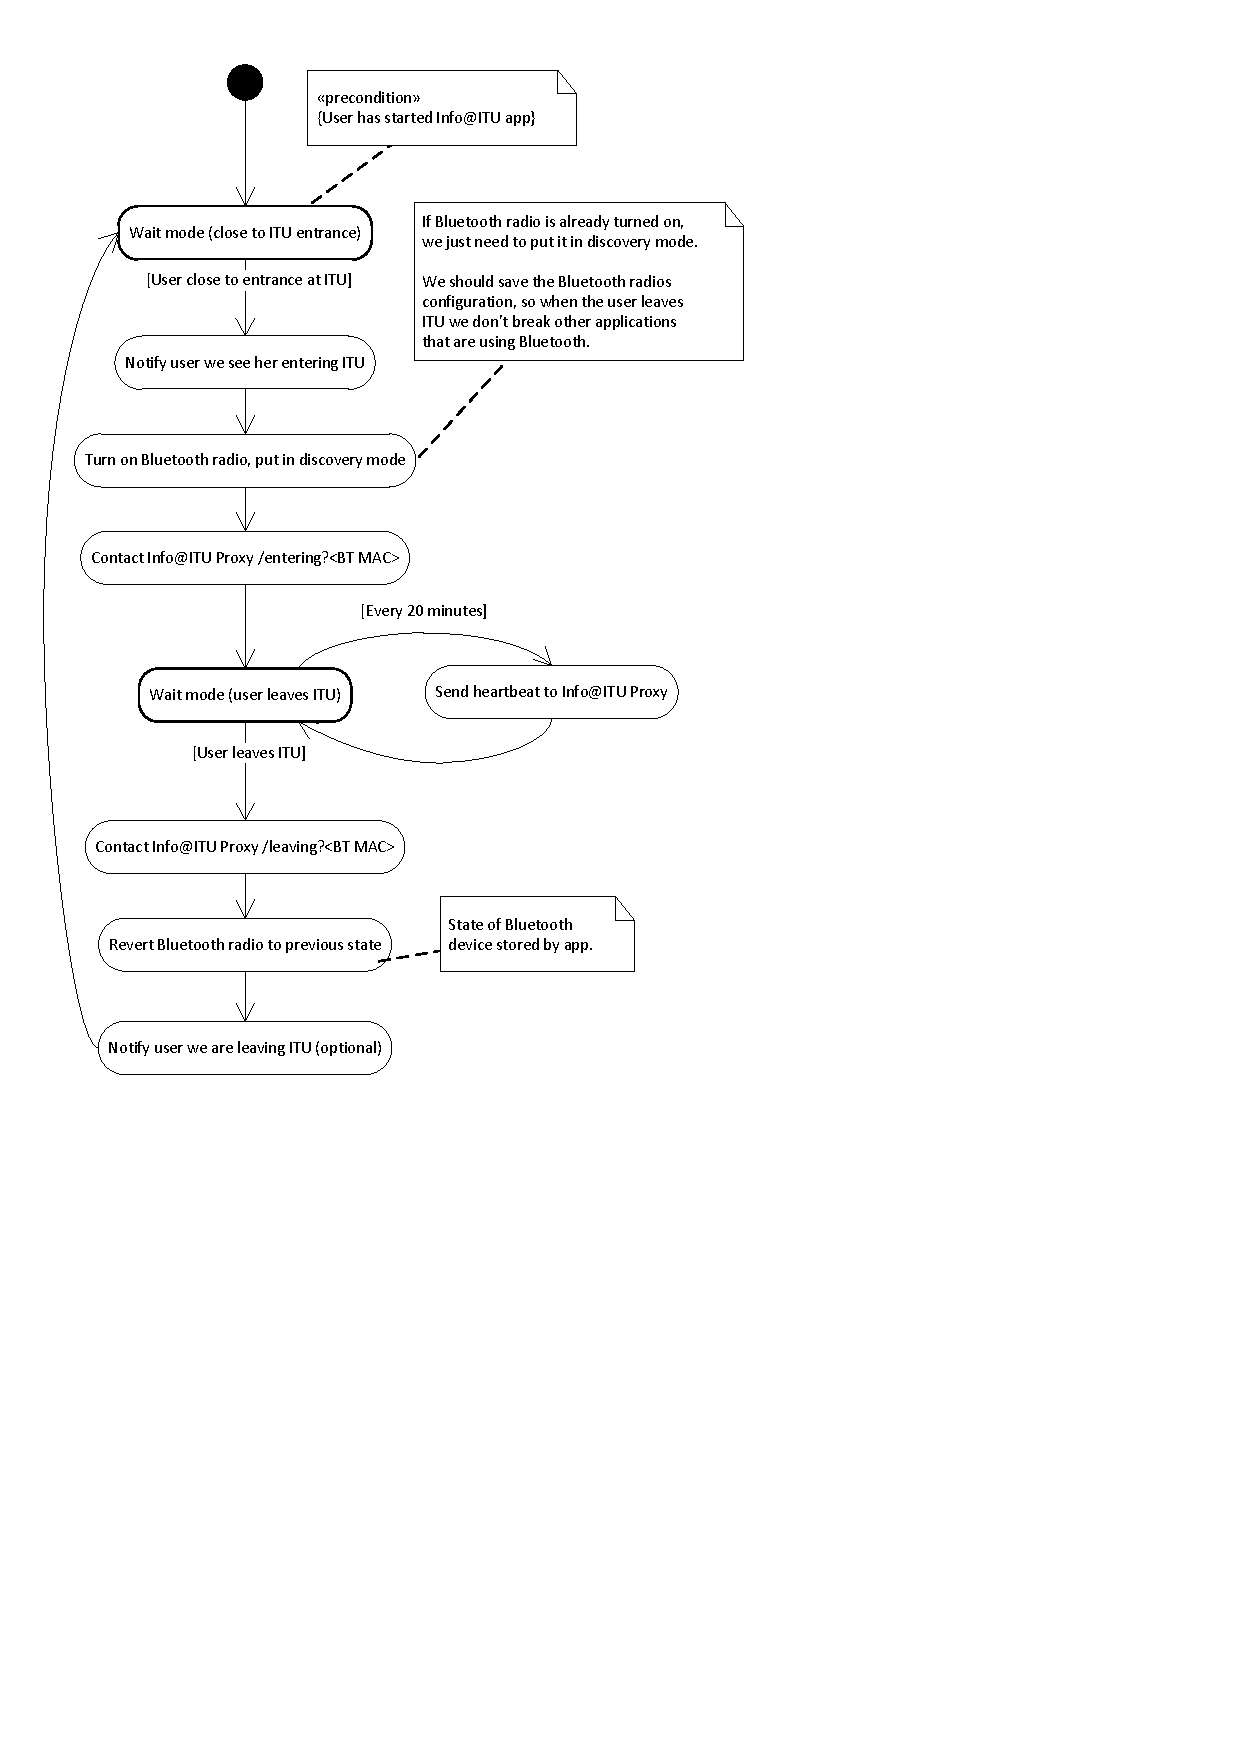
\includegraphics[width=0.90\columnwidth]{android-app-activity-diagram.pdf}
\end{center}
\caption{Activity diagram for the Info@ITU App.}
\label{fig:android-app-activity-diagram}
\end{figure}

%\bibliographystyle{abbrv}
%\bibliography{bibliography}

\end{document}